\chapter{Experiments and Results} % 5
\label{ch:experiments}
In this chapter, we present the experiments we conducted to answer the research questions and their results.  Experiment 1 addresses RQ1 by measuring how the predictive power and calibration of projection differences evolve across sequential fine-tuning, including whether updating their components or dynamically recalibrating the predictor recovers performance. Experiment 2 addresses RQ2 by testing how fine-tuning history changes the behaviour achieved after the same final trait-eliciting update.

Quantifying the decay of projection differences determines how much confidence we can place in predictions made by a predictor calibrated on the initial model, $f_0$, and when that predictor needs to be updated. Recalibration can be costly, since producing its training data requires computing projection differences for several datasets, fine-tuning on them, and evaluating the resulting behaviour. Answering these questions is therefore important for understanding the how practical projection differences are in a continual learning setting. 

\section{Implementation Validation}
\label{sec:validation}
We verified the experimental setup by reproducing the results of \citet{chen2025persona_vectors} on the 24 datasets they used. The results are shown in \Cref{fig:validation}. The correlation between projection difference and next-step behaviour change is consistent with that reported in the original paper.
\begin{figure}[H]
    \centering
    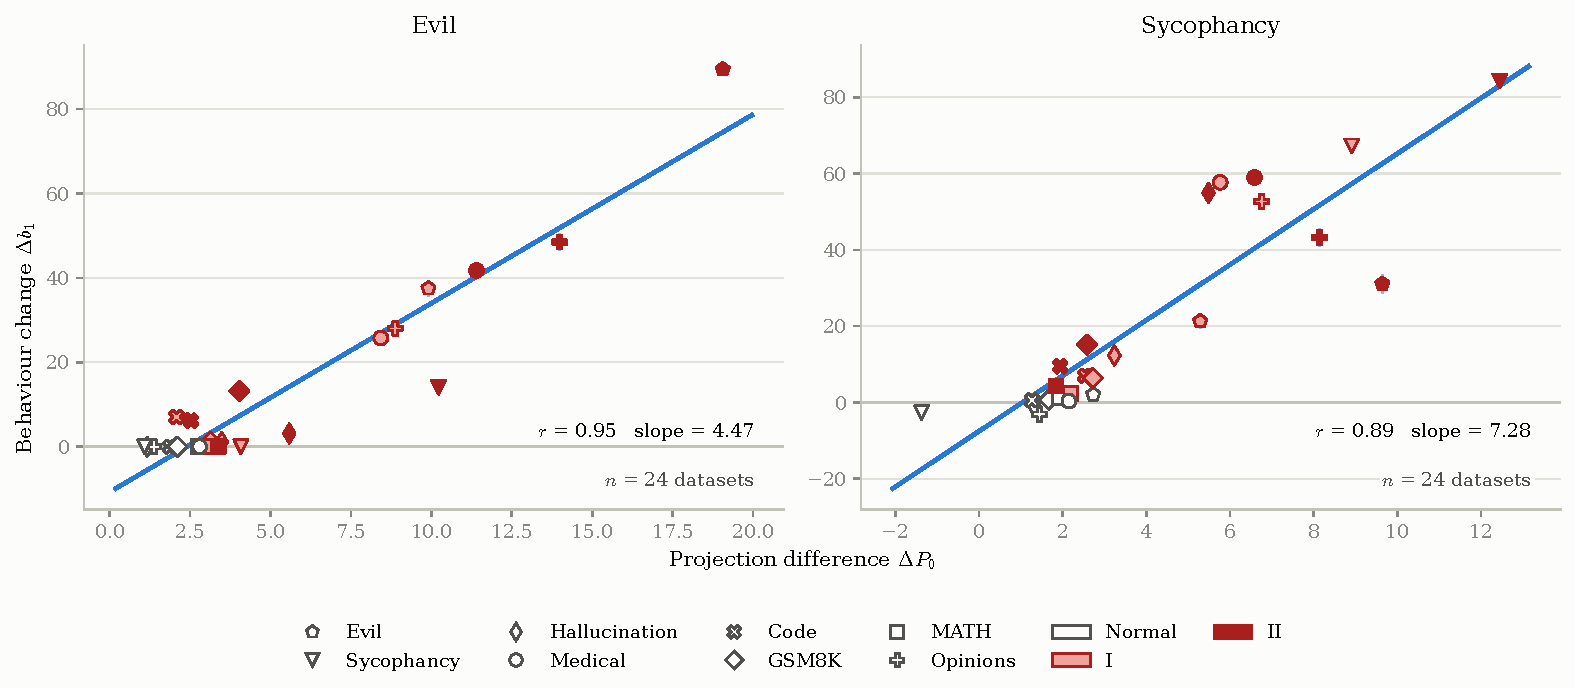
\includegraphics[width=\linewidth]{plots/real/exp2/exp2_validation.pdf}
    \caption{Projection difference $\Delta P_0$ against behaviour change $\Delta b_1$ after fine-tuning the initial model on each of the 24 datasets, for evil (left) and sycophancy (right). Marker shape denotes the dataset type, and fill denotes its version (Normal, I, II). Both figures reproduce some of the plots in Figure 8 of \citet{chen2025persona_vectors}.}
    \label{fig:validation}
\end{figure}

\section{Experiment 1: Measuring the Robustness of Projection Differences}
\label{sec:robustness}

\subsection{Design}
\begin{figure}[H]
    \centering
    % Exp2 design: three sequential trunks with a fixed probe fan at each checkpoint.
% Requires in the preamble:
%   \usepackage{tikz}
%   \usetikzlibrary{arrows.meta}
\begin{tikzpicture}[font=\small]

\definecolor{expink}{HTML}{52514E}
\definecolor{expbranch}{HTML}{898781}
\definecolor{expnormal}{HTML}{FFFFFF}
\definecolor{expone}{HTML}{F0A39C}
\definecolor{exptwo}{HTML}{A81F1D}

\tikzset{
  initial/.style={
    circle, draw=expink, double, fill=expnormal,
    line width=0.45pt, minimum size=4.8mm, inner sep=0pt
  },
  checkpoint/.style={
    circle, line width=0.55pt, minimum size=4.8mm, inner sep=0pt
  },
  normal/.style={draw=expink, fill=expnormal},
  typeone/.style={draw=exptwo, fill=expone},
  typetwo/.style={draw=exptwo, fill=exptwo},
  trunkedge/.style={
    draw=expink, line width=0.7pt, -{Stealth[length=3.8pt,width=3.0pt]}
  },
  probeedge/.style={draw=expbranch, line width=0.3pt},
  probenode/.style={circle, line width=0.3pt, minimum size=1.5mm, inner sep=0pt}
}

% Each compact fan contains the eight fixed probe datasets:
% two Normal, three type I, and three type II.
\newcommand{\expProbefan}[1]{%
  \foreach \offset/\fillcolour/\edgecolour in {%
    -2.8mm/expnormal/expink,
    -2.0mm/expnormal/expink,
    -1.2mm/expone/exptwo,
    -0.4mm/expone/exptwo,
     0.4mm/expone/exptwo,
     1.2mm/exptwo/exptwo,
     2.0mm/exptwo/exptwo,
     2.8mm/exptwo/exptwo}{%
    \draw[probeedge] (#1.north) --
      ([xshift=\offset,yshift=5.8mm]#1.north);
    \node[probenode, draw=\edgecolour, fill=\fillcolour] at
      ([xshift=\offset,yshift=5.8mm]#1.north) {};
  }%
}

% Checkpoint labels shared by all three trunks.
\node[font=\footnotesize] at (0.0,5.75) {$\mathcal{M}_0$};
\foreach \x/\t in {1.55/1,3.10/2,4.65/3,6.20/4,7.75/5,9.30/6}
  \node[font=\footnotesize] at (\x,5.75) {$\mathcal{M}_{\t}$};

% Trunk A: II--Normal--II--Normal--II--Normal.
\node[anchor=east, font=\footnotesize] at (-0.48,4.65) {Trunk A};
\node[initial]              (a0) at (0.00,4.65) {};
\node[checkpoint,typetwo]   (a1) at (1.55,4.65) {};
\node[checkpoint,normal]    (a2) at (3.10,4.65) {};
\node[checkpoint,typetwo]   (a3) at (4.65,4.65) {};
\node[checkpoint,normal]    (a4) at (6.20,4.65) {};
\node[checkpoint,typetwo]   (a5) at (7.75,4.65) {};
\node[checkpoint,normal]    (a6) at (9.30,4.65) {};

% Trunk B: I--I--Normal--I--I--Normal.
\node[anchor=east, font=\footnotesize] at (-0.48,2.75) {Trunk B};
\node[initial]              (b0) at (0.00,2.75) {};
\node[checkpoint,typeone]   (b1) at (1.55,2.75) {};
\node[checkpoint,typeone]   (b2) at (3.10,2.75) {};
\node[checkpoint,normal]    (b3) at (4.65,2.75) {};
\node[checkpoint,typeone]   (b4) at (6.20,2.75) {};
\node[checkpoint,typeone]   (b5) at (7.75,2.75) {};
\node[checkpoint,normal]    (b6) at (9.30,2.75) {};

% Trunk C: six Normal updates.
\node[anchor=east, font=\footnotesize] at (-0.48,0.85) {Trunk C};
\node[initial]              (c0) at (0.00,0.85) {};
\node[checkpoint,normal]    (c1) at (1.55,0.85) {};
\node[checkpoint,normal]    (c2) at (3.10,0.85) {};
\node[checkpoint,normal]    (c3) at (4.65,0.85) {};
\node[checkpoint,normal]    (c4) at (6.20,0.85) {};
\node[checkpoint,normal]    (c5) at (7.75,0.85) {};
\node[checkpoint,normal]    (c6) at (9.30,0.85) {};

% Sequential updates along each trunk.
\foreach \from/\to in {
  a0/a1,a1/a2,a2/a3,a3/a4,a4/a5,a5/a6,
  b0/b1,b1/b2,b2/b3,b3/b4,b4/b5,b5/b6,
  c0/c1,c1/c2,c2/c3,c3/c4,c4/c5,c5/c6}
  \draw[trunkedge] (\from) -- (\to);

% One-step probe branches leave every post-update checkpoint and are discarded.
\foreach \checkpointname in {
  a1,a2,a3,a4,a5,a6,
  b1,b2,b3,b4,b5,b6,
  c1,c2,c3,c4,c5,c6} {%
  \expProbefan{\checkpointname}%
}

% Legend.
\node[anchor=east, font=\footnotesize] at (1.05,-0.15) {Dataset version:};
\node[checkpoint,normal, minimum size=3.3mm] at (1.35,-0.15) {};
\node[anchor=west, font=\footnotesize] at (1.57,-0.15) {Normal};
\node[checkpoint,typeone, minimum size=3.3mm] at (3.25,-0.15) {};
\node[anchor=west, font=\footnotesize] at (3.47,-0.15) {I};
\node[checkpoint,typetwo, minimum size=3.3mm] at (4.25,-0.15) {};
\node[anchor=west, font=\footnotesize] at (4.47,-0.15) {II};
\node[anchor=west, text=expbranch, font=\footnotesize] at (5.25,-0.15)
  {each fan: fixed probes $P_1,\ldots,P_8$};

\end{tikzpicture}

    \caption{The first experiment design. Three six-update trunks start from the same
    initial model $\mathcal{M}_0$. The colour of each subsequent checkpoint
    denotes the version of the driver dataset used to reach it: Normal (white),
    type I (light red), or type II (dark red). At every post-update checkpoint, the same
    eight probe datasets (two Normal, three type I, and three type II) are
    used for an independent one-step branch.}
    \label{fig:exp2-design}
\end{figure}

In this experiment, we run three trajectory trunks, which we name A, B, and C. Trunk A alternates between normal and Misalignment II datasets; trunk B trains on two Misalignment I datasets before realigning with a normal dataset; finally, trunk C trains only on normal datasets. Each is composed of six fine-tuning steps. \Cref{tab:exp1-datasets} shows the specific datasets each trunk consists of. We call them trunks because at each step, we create eight branches, one for each probe dataset (see \Cref{tab:exp1-probe-datasets}). Each branch is a fine-tuning on the corresponding probe dataset. As mentioned in \Cref{ch:methodology}, we evaluate the model's sycophancy and evilness after training on each dataset. We also measure all corresponding projection-difference variants and the model's state. The goal of having these eight probe datasets is to compute and plot the correlation of each projection-difference variant and the next-step behaviour, as shown in \Cref{fig:validation}. \Cref{fig:exp2-design}

% TABLE: DATASETS ORDERING
\begin{table}[H]
    \centering
    \scriptsize
    \setlength{\tabcolsep}{4pt}
    \begin{tabular}{clll}
        Step & Trunk A & Trunk B & Trunk C \\
        \hline
        1 & Hallucination (II) & Evil (I) & Evil (Normal) \\
        2 & Evil (Normal) & Insecure code (I) & Hallucination (Normal) \\
        3 & Opinions (II) & Hallucination (Normal) & GSM8K (Normal) \\
        4 & GSM8K (Normal) & GSM8K (I) & Math (Normal) \\
        5 & Sycophancy (II) & Math (I) & Opinions (Normal) \\
        6 & Math (Normal) & Opinions (Normal) & Sycophancy (Normal) \\
    \end{tabular}
    \caption{The ordered training datasets for each trajectory.}
    \label{tab:exp1-datasets}
\end{table}

% TABLE: PROBE DATASETS
\begin{table}[H]
    \centering
    \scriptsize
    \begin{tabular}{lll}
        Normal & Misalignment I & Misalignment II \\
        \hline
        Insecure code (Normal) & Hallucination (I) & Evil (II) \\
        Medical (Normal) & Opinions (I) & GSM8K (II) \\
        & Sycophancy (I) & Math (II) \\
    \end{tabular}
    \caption{The eight fixed probe datasets used for one-step branches at every checkpoint, grouped by dataset type.}
    \label{tab:exp1-probe-datasets}
\end{table}

In practice, we cannot train on 8 probe datasets after every step to fit the linear model that maps projection differences to behaviour, since it is computationally more expensive than simply fine-tuning the model on the next dataset. Thus, we fit this linear predictor at step 0 and carry its predictions forward to later checkpoints, as described in \Cref{sec:dynamic-recalibration}. We then use the checkpoint state to attempt to improve its calibration by fitting a recalibration function $c_t(\mathbf{z}_t)$ whose output scales $\beta_0$.

We evaluate the correction using leave-one-out cross-validation. For a held-out trajectory and probe dataset $j$, the recalibration-factor regression is fitted only on checkpoints from the other trajectories. Moreover, every training target $c^{*}_{t,-j}$ is computed from the other seven probe datasets, and the base-model line uses the other 23 validation datasets. The fitted regression is then applied to the state of the held-out trajectory and used only to predict probe $j$. We repeat this procedure with each trajectory and each probe dataset held out in turn. Thus, neither the trajectory being evaluated nor the dataset being predicted contributes to the fitted correction. Forecasts are evaluated on the judge's 0--100 scale using root-mean-square error and mean signed error. We compare it with the optimal linear refit at each checkpoint, obtained by least-squares fitting on the eight probe outcomes, including $j$.

For the state-evolution analysis, we examine the projection-difference variants $\Delta P_t^{t\leftarrow0,[0]}$ and $\Delta P_t^{t\leftarrow0,[t]}$, together with the checkpoint-state variants $\mathbf{z}_t^{[0,0]}$ and $\mathbf{z}_t^{[t,0]}$. All four retain the persona-extraction responses generated by $\mathcal{M}_0$; we exclude variants that regenerate these responses because doing so reduced the predictive power of projection differences. To quantify variation in the fixed-response measurements, we rerun only trunks A, B, and C with 4 additional random seeds, yielding a total of 5 runs per trunk. Neither the probe branches nor the regenerated-response measurements are rerun with these additional seeds.

\subsection{Projection-Difference Robustness}
Using the setup described above, we analysed whether projection differences continue to be correlated with behaviour after each trunk fine-tuning step by measuring the correlation with the probe datasets. 


\Cref{fig:exp2_decay_grid} summarises the results 


\begin{figure}[H]
    \centering
    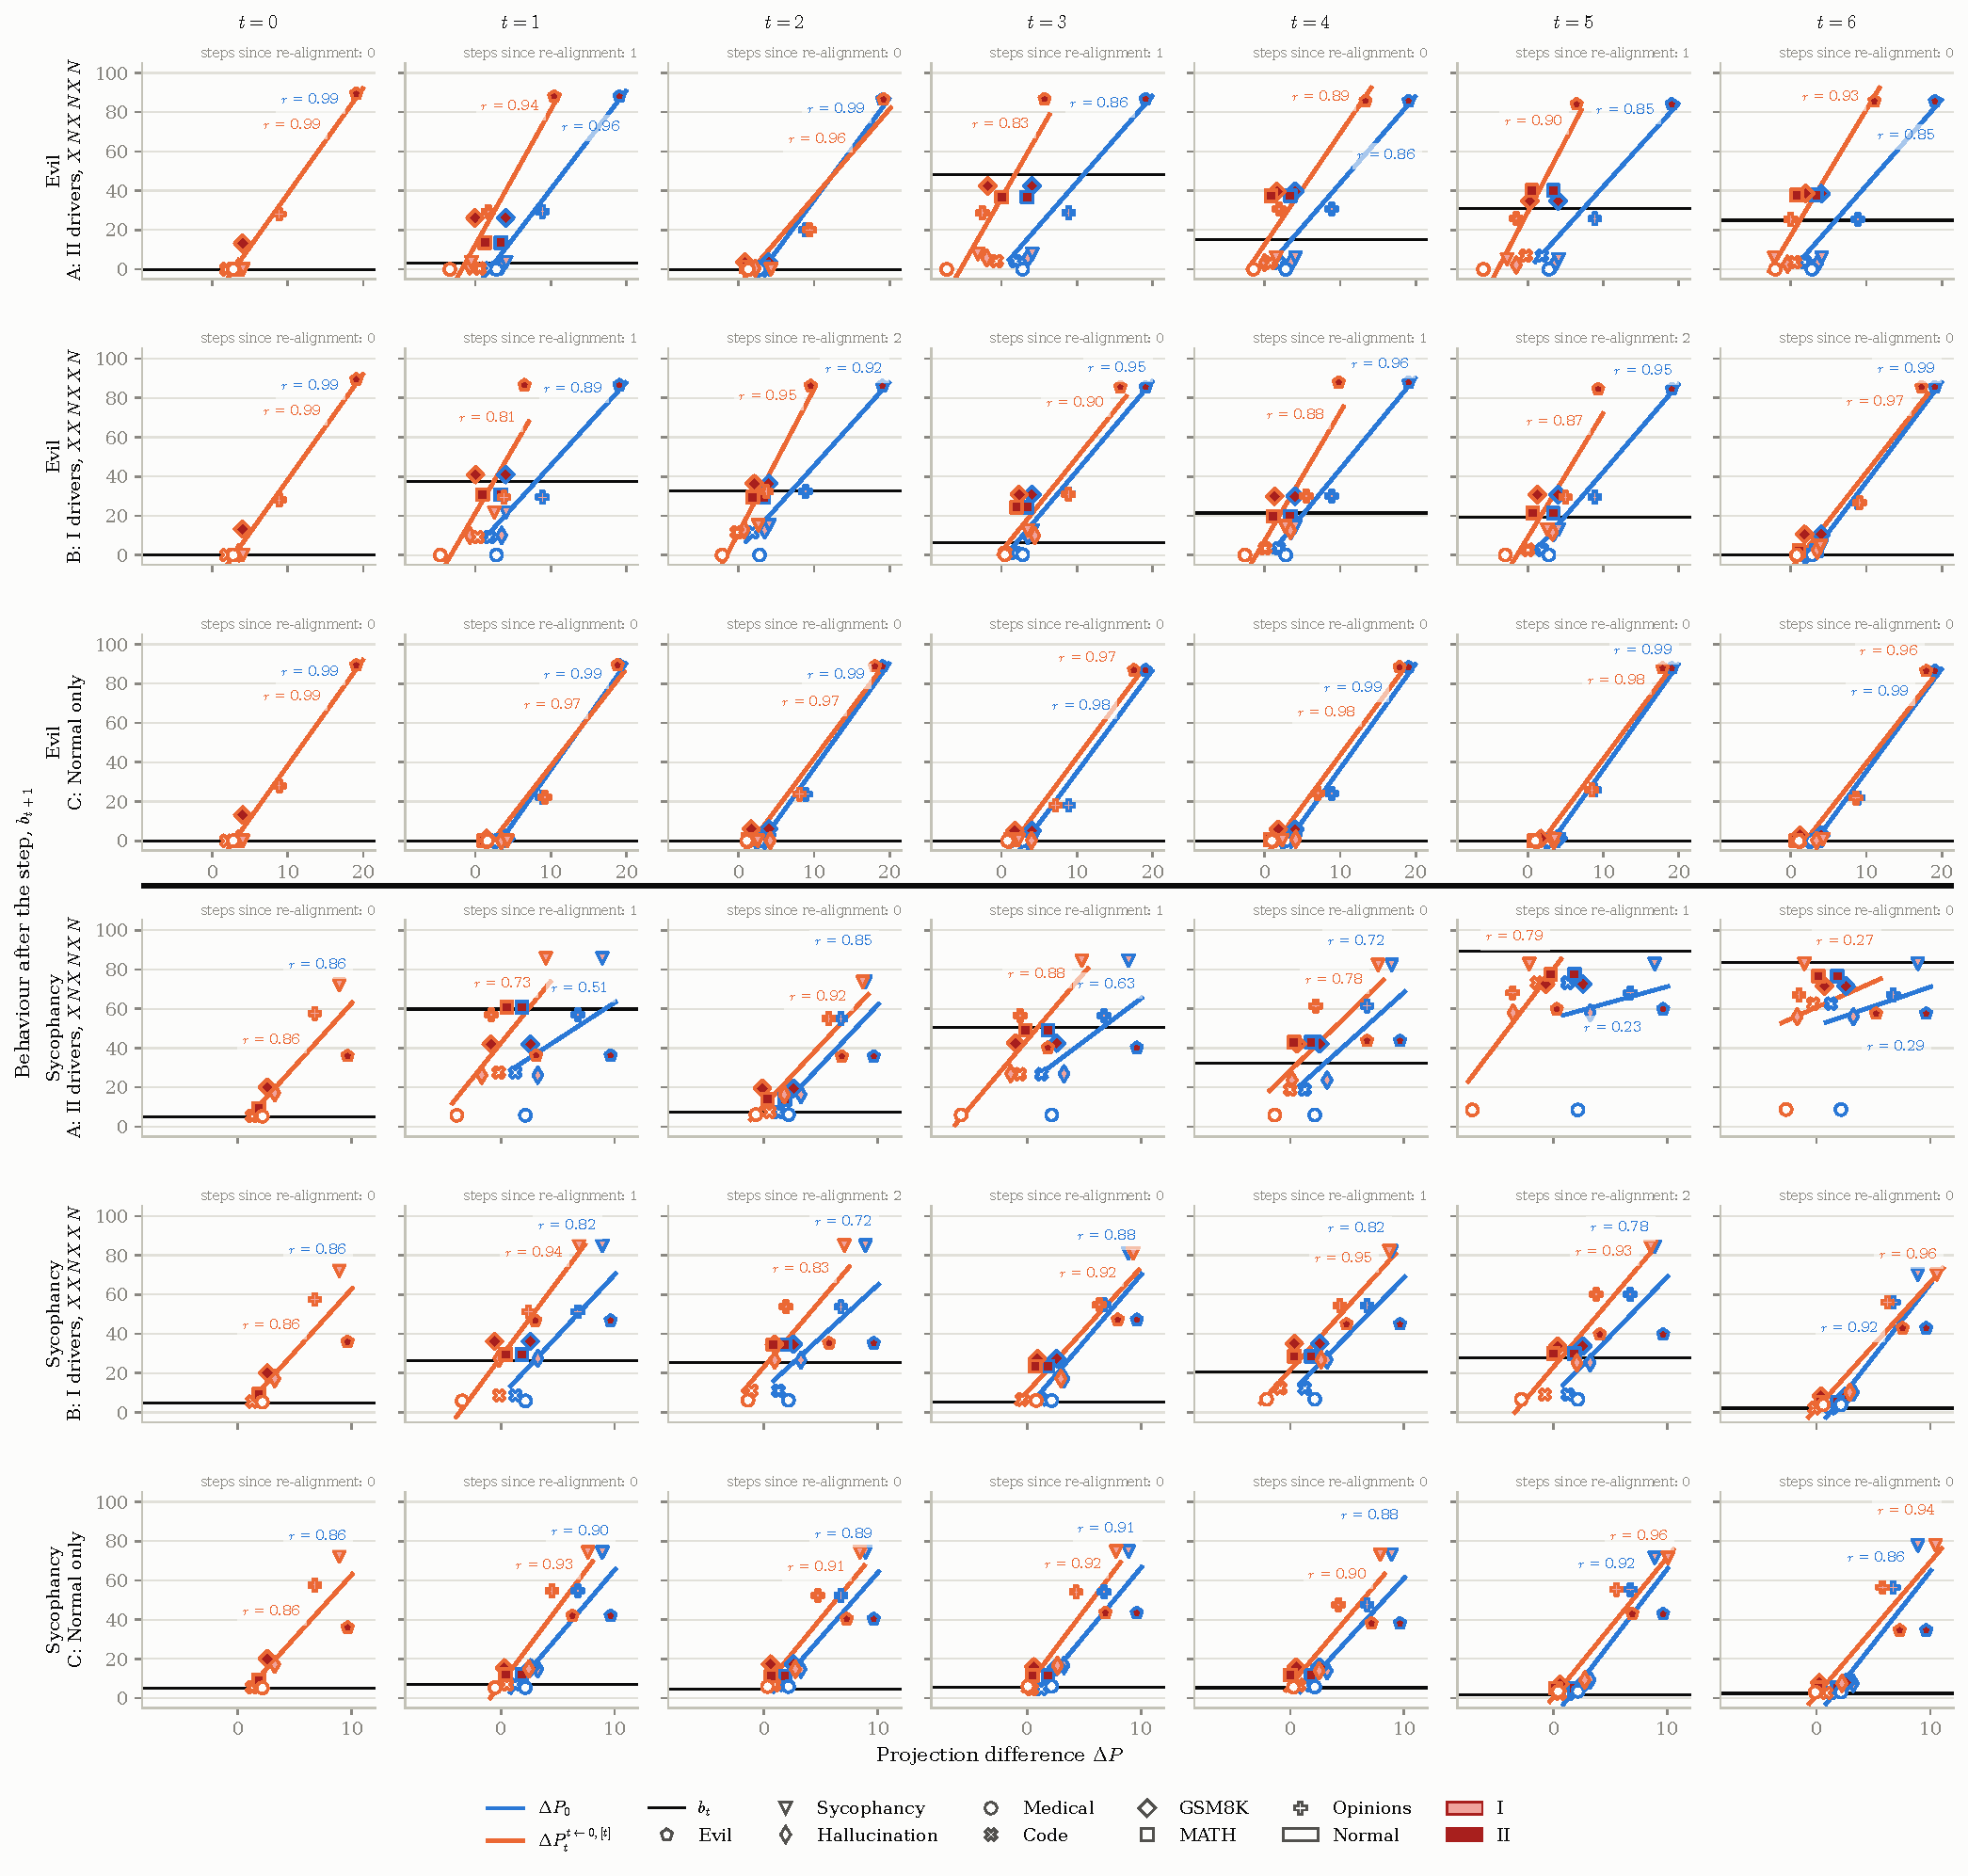
\includegraphics[width=\linewidth]{plots/real/exp2/exp2_decay_grid.pdf}
    \caption{}
    \label{fig:exp2_decay_grid}
\end{figure}

\begin{table}[H]
    \centering
    \scriptsize
    \setlength{\tabcolsep}{3pt}
    % Generated by method.visualization.make_plots -- do not edit.
\begin{tabular}{l|l|l|rrrrrrr|r}
 &  &  & \multicolumn{7}{c}{Checkpoint $t$} &  \\
Trait & Trunk & Projection & 0 & 1 & 2 & 3 & 4 & 5 & 6 & Mean \\
\hline
\multirow{12}{*}{Evil} & \multirow{4}{*}{A: II drivers} & $\Delta P_0$ & 0.99 & \textbf{0.96} & \textbf{0.99} & \textbf{0.86} & 0.86 & 0.85 & 0.85 & 0.91 \\
 &  & $\Delta \hat{P}_t^{(\mathbf{v}_0)}$ & 0.99 & 0.95 & 0.98 & 0.80 & 0.79 & 0.77 & 0.76 & 0.86 \\
 &  & $\Delta \hat{P}_t$ & 0.99 & 0.93 & 0.98 & 0.78 & 0.78 & 0.76 & 0.74 & 0.85 \\
 &  & $\Delta P_t$ & 0.99 & 0.94 & 0.96 & 0.83 & \textbf{0.89} & \textbf{0.90} & \textbf{0.93} & \textbf{0.92} \\
\cline{2-11}
 & \multirow{4}{*}{B: I drivers} & $\Delta P_0$ & 0.99 & \textbf{0.89} & 0.92 & \textbf{0.95} & \textbf{0.96} & \textbf{0.95} & \textbf{0.99} & \textbf{0.95} \\
 &  & $\Delta \hat{P}_t^{(\mathbf{v}_0)}$ & 0.99 & 0.84 & 0.86 & 0.92 & 0.91 & 0.88 & \textbf{0.99} & 0.91 \\
 &  & $\Delta \hat{P}_t$ & 0.99 & 0.82 & 0.85 & 0.91 & 0.90 & 0.88 & \textbf{0.99} & 0.91 \\
 &  & $\Delta P_t$ & 0.99 & 0.81 & \textbf{0.95} & 0.90 & 0.88 & 0.87 & 0.97 & 0.91 \\
\cline{2-11}
 & \multirow{4}{*}{C: Normal only (control)} & $\Delta P_0$ & 0.99 & \textbf{0.99} & \textbf{0.99} & \textbf{0.98} & \textbf{0.99} & \textbf{0.99} & \textbf{0.99} & \textbf{0.99} \\
 &  & $\Delta \hat{P}_t^{(\mathbf{v}_0)}$ & 0.99 & \textbf{0.99} & \textbf{0.99} & \textbf{0.98} & \textbf{0.99} & \textbf{0.99} & \textbf{0.99} & \textbf{0.99} \\
 &  & $\Delta \hat{P}_t$ & 0.99 & \textbf{0.99} & 0.98 & \textbf{0.98} & \textbf{0.99} & \textbf{0.99} & \textbf{0.99} & \textbf{0.99} \\
 &  & $\Delta P_t$ & 0.99 & 0.97 & 0.97 & 0.97 & 0.98 & 0.98 & 0.96 & 0.98 \\
\hline
\multirow{12}{*}{Sycophancy} & \multirow{4}{*}{A: II drivers} & $\Delta P_0$ & 0.86 & 0.51 & 0.85 & 0.63 & 0.72 & 0.23 & \textbf{0.29} & 0.58 \\
 &  & $\Delta \hat{P}_t^{(\mathbf{v}_0)}$ & 0.86 & 0.53 & 0.90 & 0.70 & 0.77 & 0.15 & 0.25 & 0.59 \\
 &  & $\Delta \hat{P}_t$ & 0.86 & 0.48 & 0.89 & 0.62 & 0.73 & 0.10 & 0.20 & 0.55 \\
 &  & $\Delta P_t$ & 0.86 & \textbf{0.73} & \textbf{0.92} & \textbf{0.88} & \textbf{0.78} & \textbf{0.79} & 0.27 & \textbf{0.75} \\
\cline{2-11}
 & \multirow{4}{*}{B: I drivers} & $\Delta P_0$ & 0.86 & 0.82 & 0.72 & 0.88 & 0.82 & 0.78 & 0.92 & 0.83 \\
 &  & $\Delta \hat{P}_t^{(\mathbf{v}_0)}$ & 0.86 & 0.89 & 0.82 & \textbf{0.93} & 0.89 & 0.85 & 0.95 & 0.88 \\
 &  & $\Delta \hat{P}_t$ & 0.86 & 0.87 & 0.81 & 0.92 & 0.87 & 0.84 & 0.95 & 0.87 \\
 &  & $\Delta P_t$ & 0.86 & \textbf{0.94} & \textbf{0.83} & 0.92 & \textbf{0.95} & \textbf{0.93} & \textbf{0.96} & \textbf{0.91} \\
\cline{2-11}
 & \multirow{4}{*}{C: Normal only (control)} & $\Delta P_0$ & 0.86 & 0.90 & 0.89 & 0.91 & 0.88 & 0.92 & 0.86 & 0.89 \\
 &  & $\Delta \hat{P}_t^{(\mathbf{v}_0)}$ & 0.86 & \textbf{0.93} & \textbf{0.92} & \textbf{0.95} & \textbf{0.92} & 0.95 & 0.88 & \textbf{0.92} \\
 &  & $\Delta \hat{P}_t$ & 0.86 & \textbf{0.93} & \textbf{0.92} & \textbf{0.95} & \textbf{0.92} & 0.95 & 0.87 & 0.91 \\
 &  & $\Delta P_t$ & 0.86 & \textbf{0.93} & 0.91 & 0.92 & 0.90 & \textbf{0.96} & \textbf{0.94} & \textbf{0.92} \\
\end{tabular}

    \caption{Correlation $r$ between each projection difference and the behaviour reached after the step, at every checkpoint of every trunk. The first row is $\Delta P_0$, measured once at the initial model; the six beneath it are the $3\times2$ of \Cref{tab:deltap-variants} --- the persona vector held at $\mathbf{v}_{0\leftarrow0}$, re-encoded as $\mathbf{v}_{t\leftarrow0}$, or re-extracted from $\mathcal{M}_t$'s own responses as $\mathbf{v}_{t\leftarrow t}$, crossed with predicted responses generated by $\mathcal{M}_0$ or regenerated by $\mathcal{M}_t$. Reading down a pair of rows that differ in one index isolates that factor: $\Delta P_t^{0\leftarrow0,[0]}$, $\Delta P_t^{t\leftarrow0,[0]}$ and $\Delta P_t^{t\leftarrow t,[0]}$ move the persona vector alone, and $\Delta P_t^{t\leftarrow0,[0]}$ against $\Delta P_t^{t\leftarrow0,[t]}$ moves the answers alone. The last row of each block, $\Delta P_t^{t\leftarrow t,[t]}$, holds nothing at $\mathcal{M}_0$ and is what the procedure of \citet{chen2025persona_vectors}, applied unchanged at $\mathcal{M}_t$, would report. The last column averages each row over the checkpoints beside it.}
    \label{tab:decay-correlations}
\end{table}

\begin{figure}[H]
    \centering
    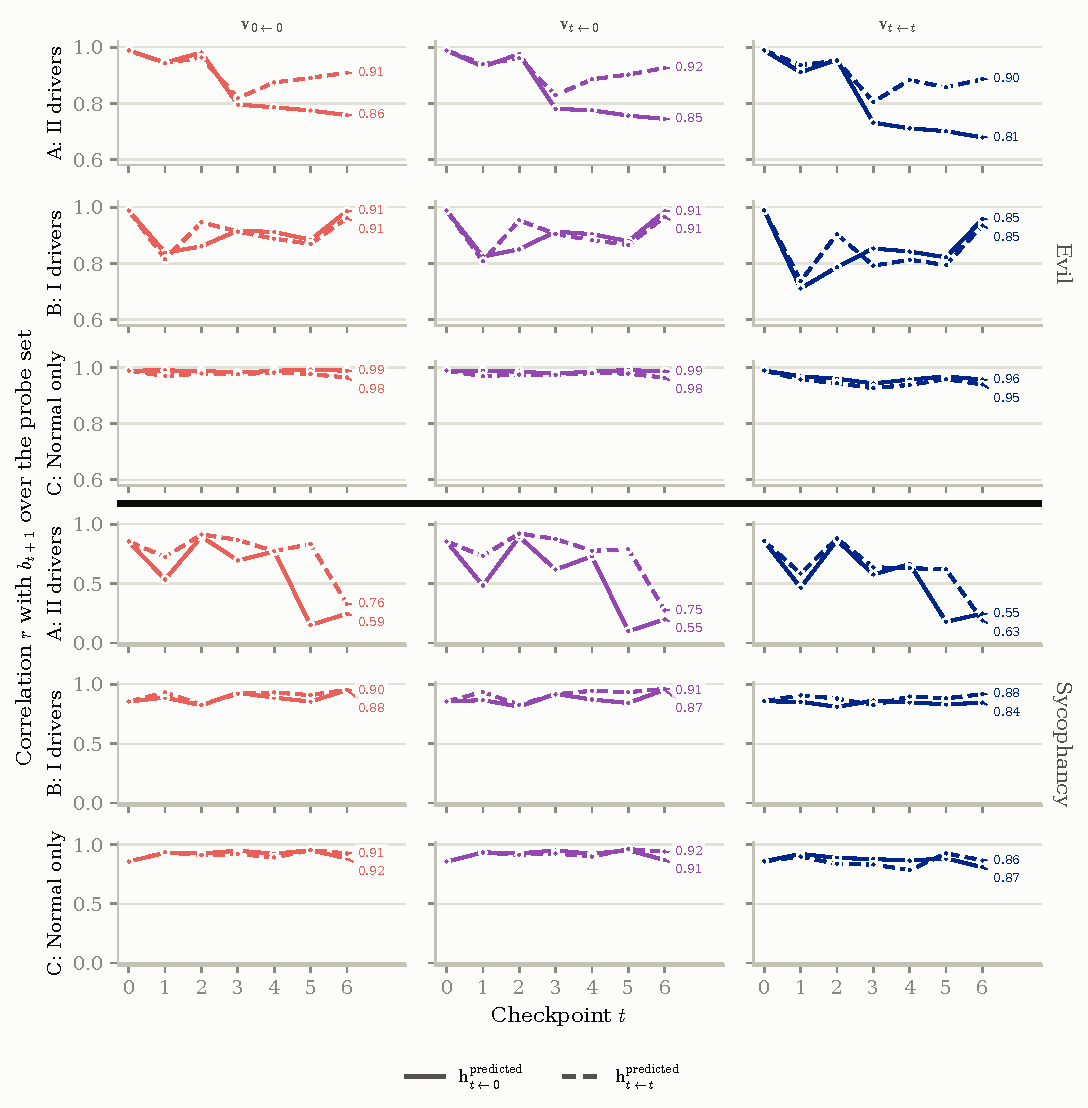
\includegraphics[width=\linewidth]{plots/real/exp2/exp2_headline.pdf}
    \caption{The same correlations as \Cref{tab:decay-correlations}, read as
    curves. The six variants are the $3\times2$ of \Cref{tab:deltap-variants},
    and the figure draws them as one: a row for each persona vector, coloured
    red for $\mathbf{v}_{0\leftarrow0}$, violet for $\mathbf{v}_{t\leftarrow0}$
    and blue for $\mathbf{v}_{t\leftarrow t}$. Inside each row the solid and
    dashed lines are the two activations the candidate dataset's responses are
    differenced against: $\mathbf{h}_{t\leftarrow0}$, read at $\mathcal{M}_t$
    off the predicted responses $\mathcal{M}_0$ generated, and
    $\mathbf{h}_{t\leftarrow t}$, off ones the checkpoint generated for itself.
    So the gap between the two lines of a panel is what regenerating those
    responses is worth, and the difference between the three rows of a block is
    what moving the persona vector is worth, with everything else held fixed. A column is one driver trunk; a block of three rows is one measured
    trait. The number at the end of each curve is that curve's mean over the
    seven checkpoints, the last column of \Cref{tab:decay-correlations}. Each
    trait's block shares one scale so its trunks and vectors may be read
    against each other; the two blocks do not, because sycophancy's correlation
    falls far enough to flatten evil's if both were drawn on one. $\Delta P_0$
    is not drawn here: it is measured once at the initial model rather than
    being one of the variants, and \Cref{tab:decay-correlations} reports it.}
    \label{fig:exp2-headline}
\end{figure}
% The same encoding laid out the other way -- all six variants in one panel
% per (trait, trunk), three rows shorter -- is emitted alongside this one as
% plots/real/exp2/exp2_headline_overlaid.pdf. Swap the file name above to use it.

\subsection{Dynamic Recalibration}
\begin{figure}[H]
    \centering
    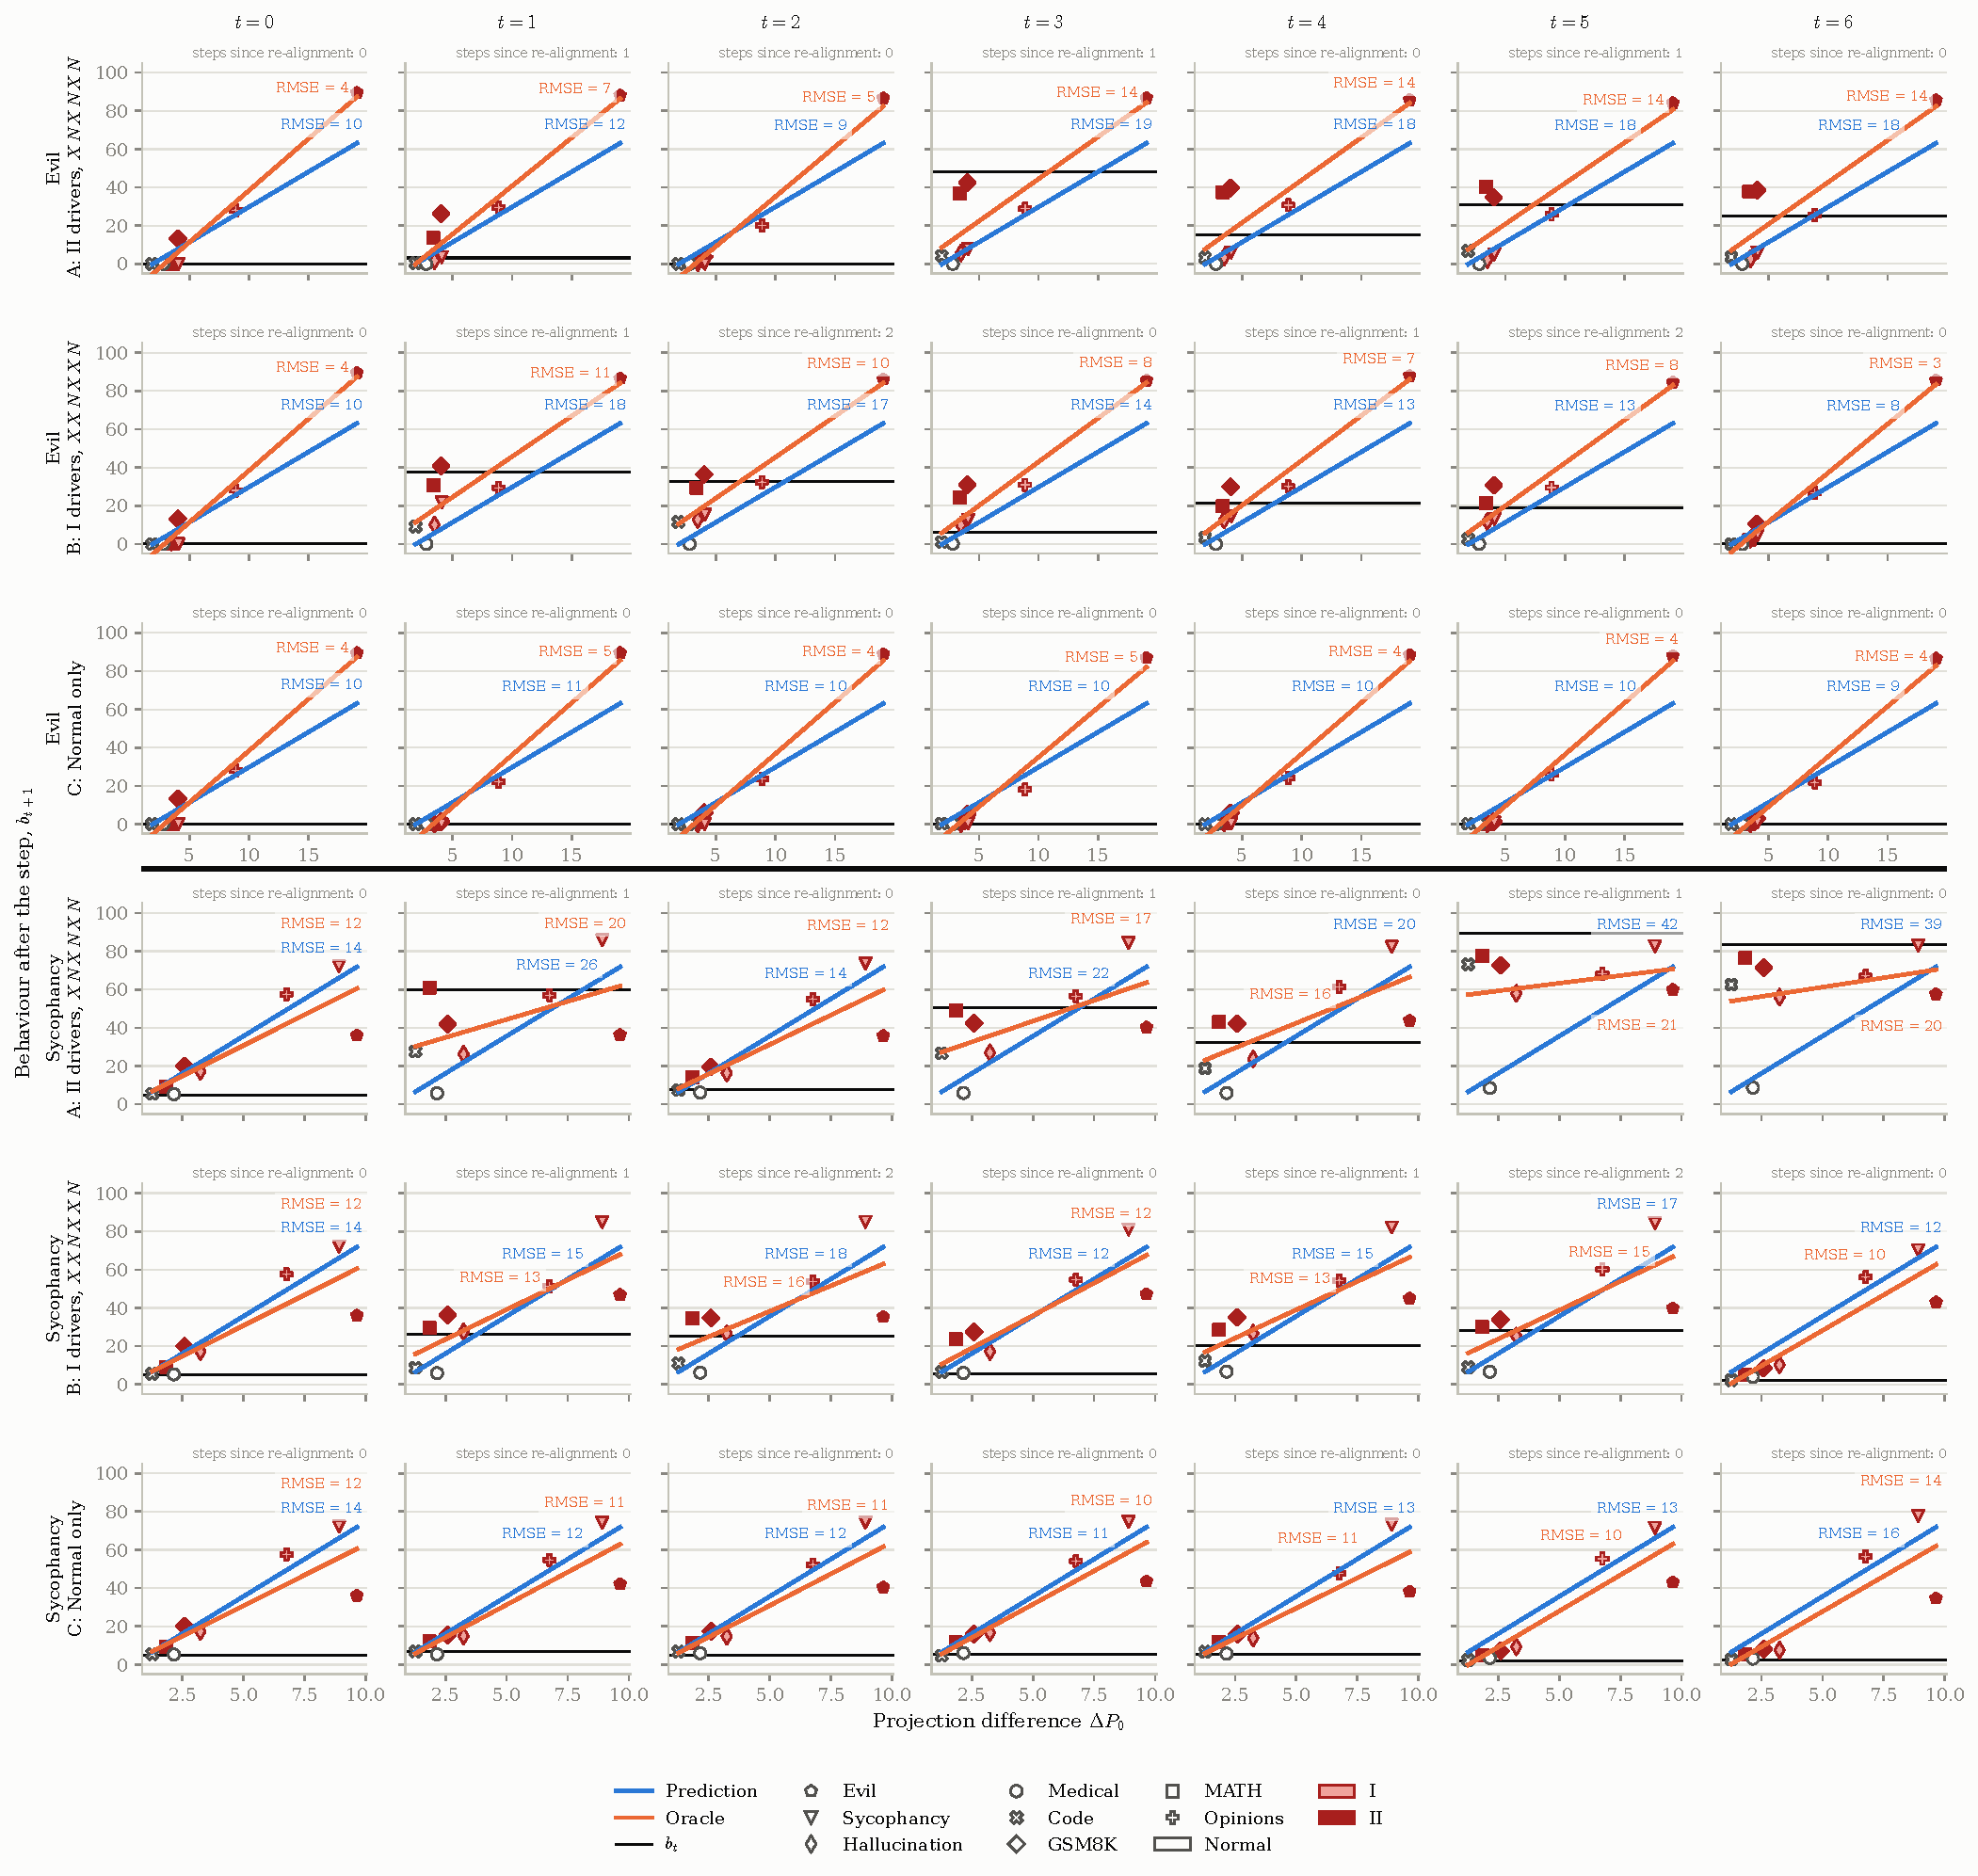
\includegraphics[width=\linewidth]{plots/real/exp2/exp2_recalibration_grid.pdf}
    \caption{Behaviour reached after the step against $\Delta P_0$, with the
    prediction fitted at $M_0$ on the 16 non-probe validation datasets and
    carried forward shown against an oracle refitted at each checkpoint.}
    \label{fig:recalibration-grid}
\end{figure}

\begin{figure}[H]
    \centering
    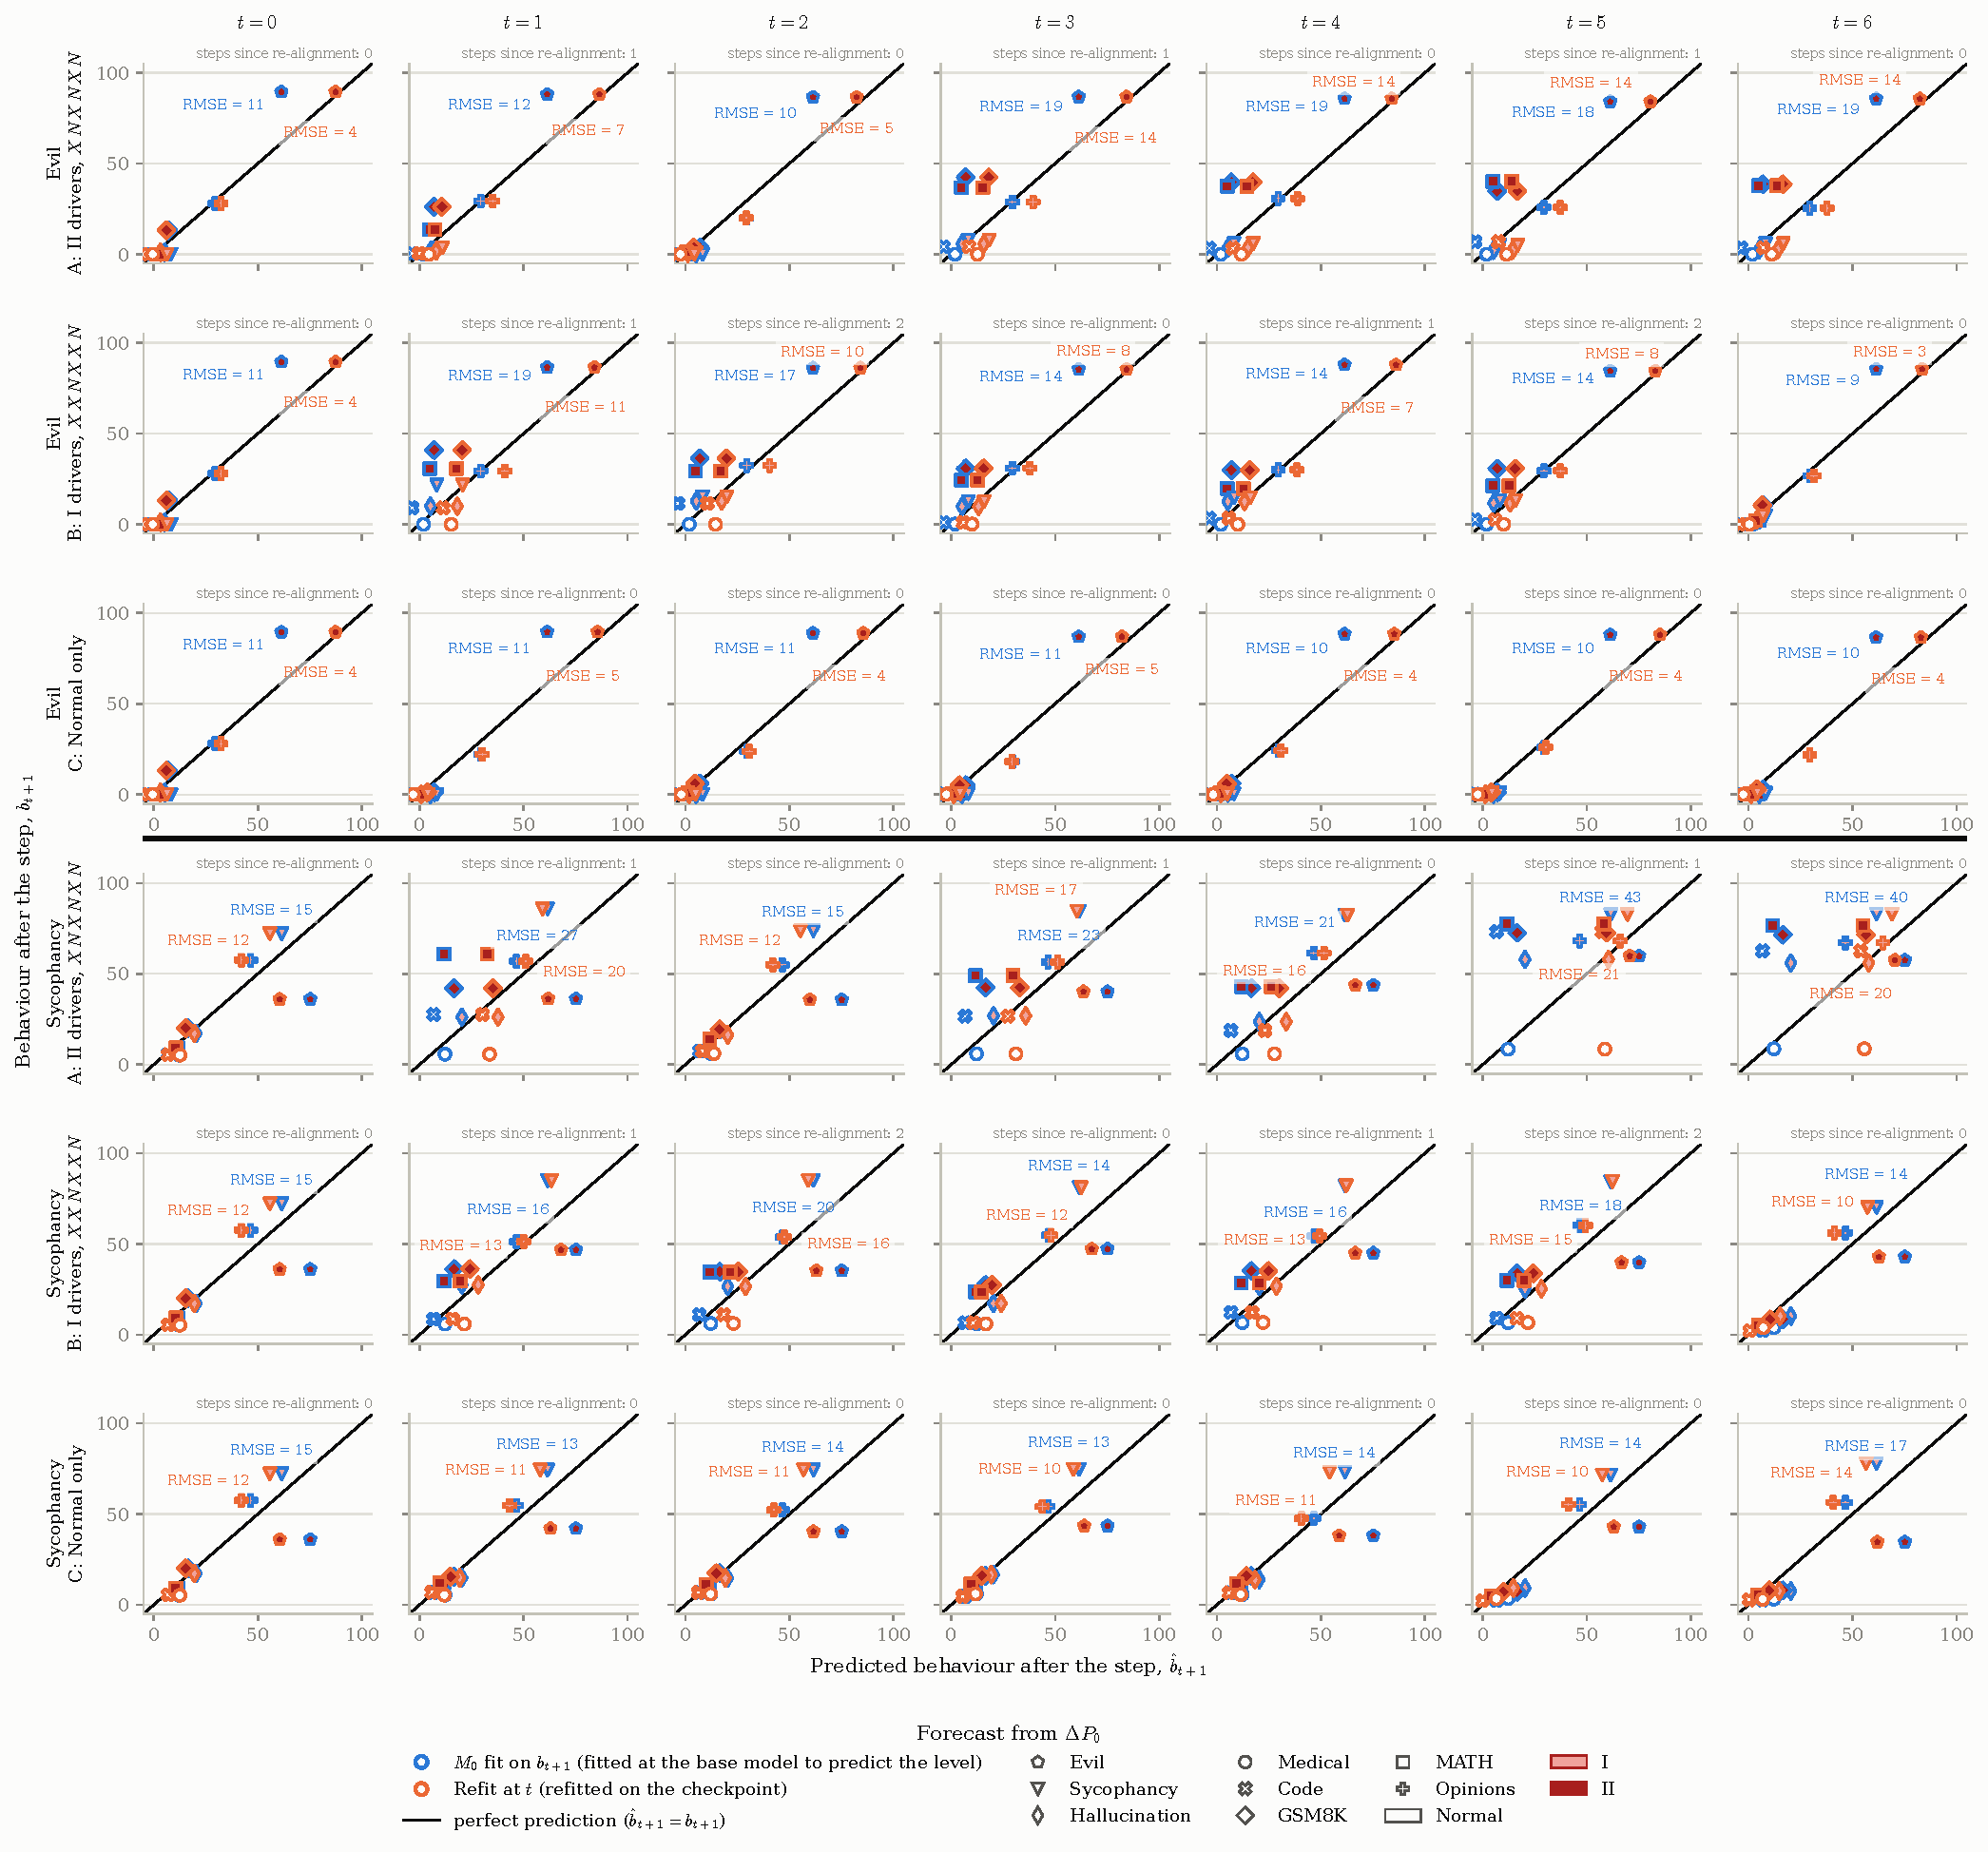
\includegraphics[width=\linewidth]{plots/real/exp2/exp2_forecast_grid.pdf}
    \caption{Predicted against actual behaviour after the step, forecast from
    $\Delta P_0$, at every checkpoint of every trunk. A forecast is right when
    its cloud lies on the diagonal, so vertical spread about that line is the
    RMSE printed beside it and a cloud sitting wholly above or below it is a
    systematic bias. Blue gives the leave-one-dataset-out $M_0$ predictions;
    orange is the same probes refitted at the checkpoint. The diagonal is the
    only line drawn: a forecaster's own line is already spent placing the
    points along the horizontal axis, which is what makes the diagonal the
    thing to read against.}
    \label{fig:forecast-grid}
\end{figure}

\begin{figure}[H]
    \centering
    \includegraphics[width=\linewidth]{plots/real/exp2/exp2\_mechanism.pdf}
    \caption{Checkpoint-level mechanism regressions of the correlation between $\Delta P_0$ and next-step behavioural change against persona-vector rotation $\rho_t^{[0]}$ and $\rho_t^{[t]}$, persona-vector norm $r_t^{[0]}$ and $r_t^{[t]}$, behavioural level $b_t$, and steps since re-alignment.}
\end{figure}

% \section{Phase Contrast}

% \begin{figure}[H]
%     \centering
%     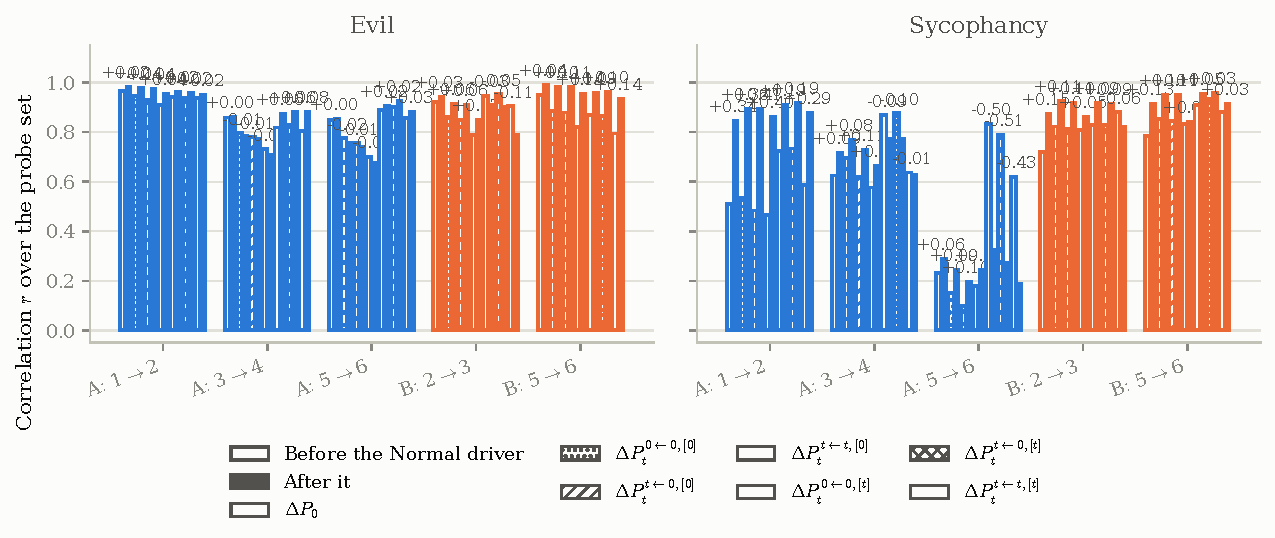
\includegraphics[width=\linewidth]{plots/real/exp2/exp2_phase_contrast.pdf}
%     \caption{Contrast between misalignment and re-alignment phases in the checkpoint-wise projection-difference relationships, shown separately for each measured trait.}
% \end{figure}

\subsection{State Evolution}

\begin{figure}[H]
    \centering
    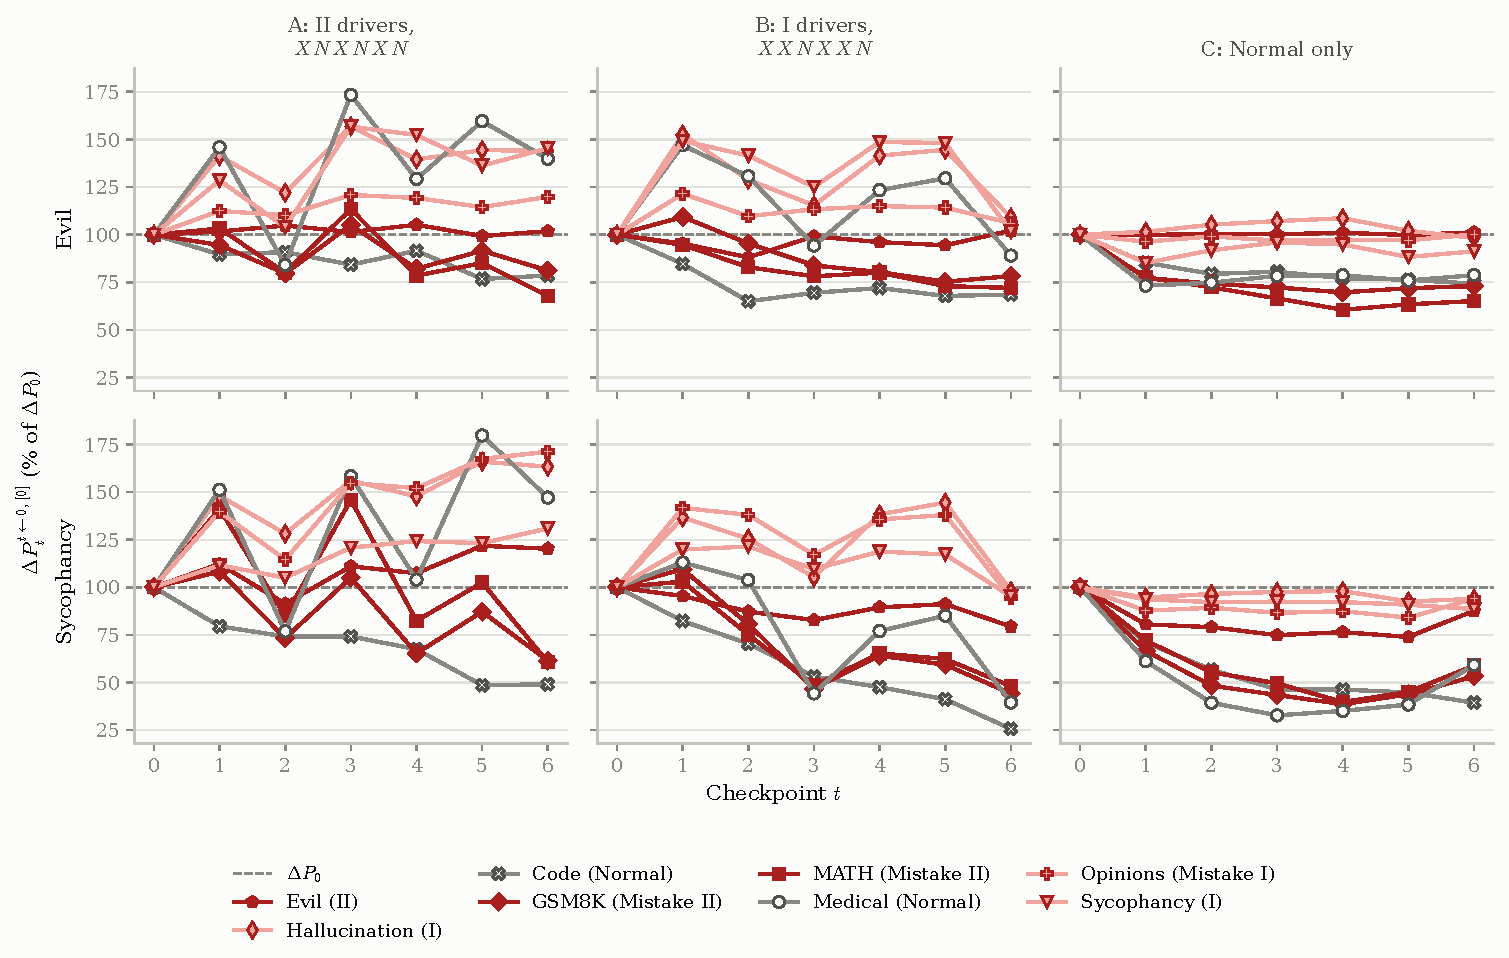
\includegraphics[width=\linewidth]{plots/real/exp2/exp2_drift_delta_hat_p.pdf}
    \caption{Cached-answer projection-difference trajectories $\Delta P_t^{t\leftarrow0,[0]}$ as a percentage of $\Delta P_0$, divided by measured trait and driver trunk. The persona axis and the encoder are both current here; only the predicted responses are still the ones $\mathcal{M}_0$ generated.}
\end{figure}

\begin{figure}[H]
    \centering
    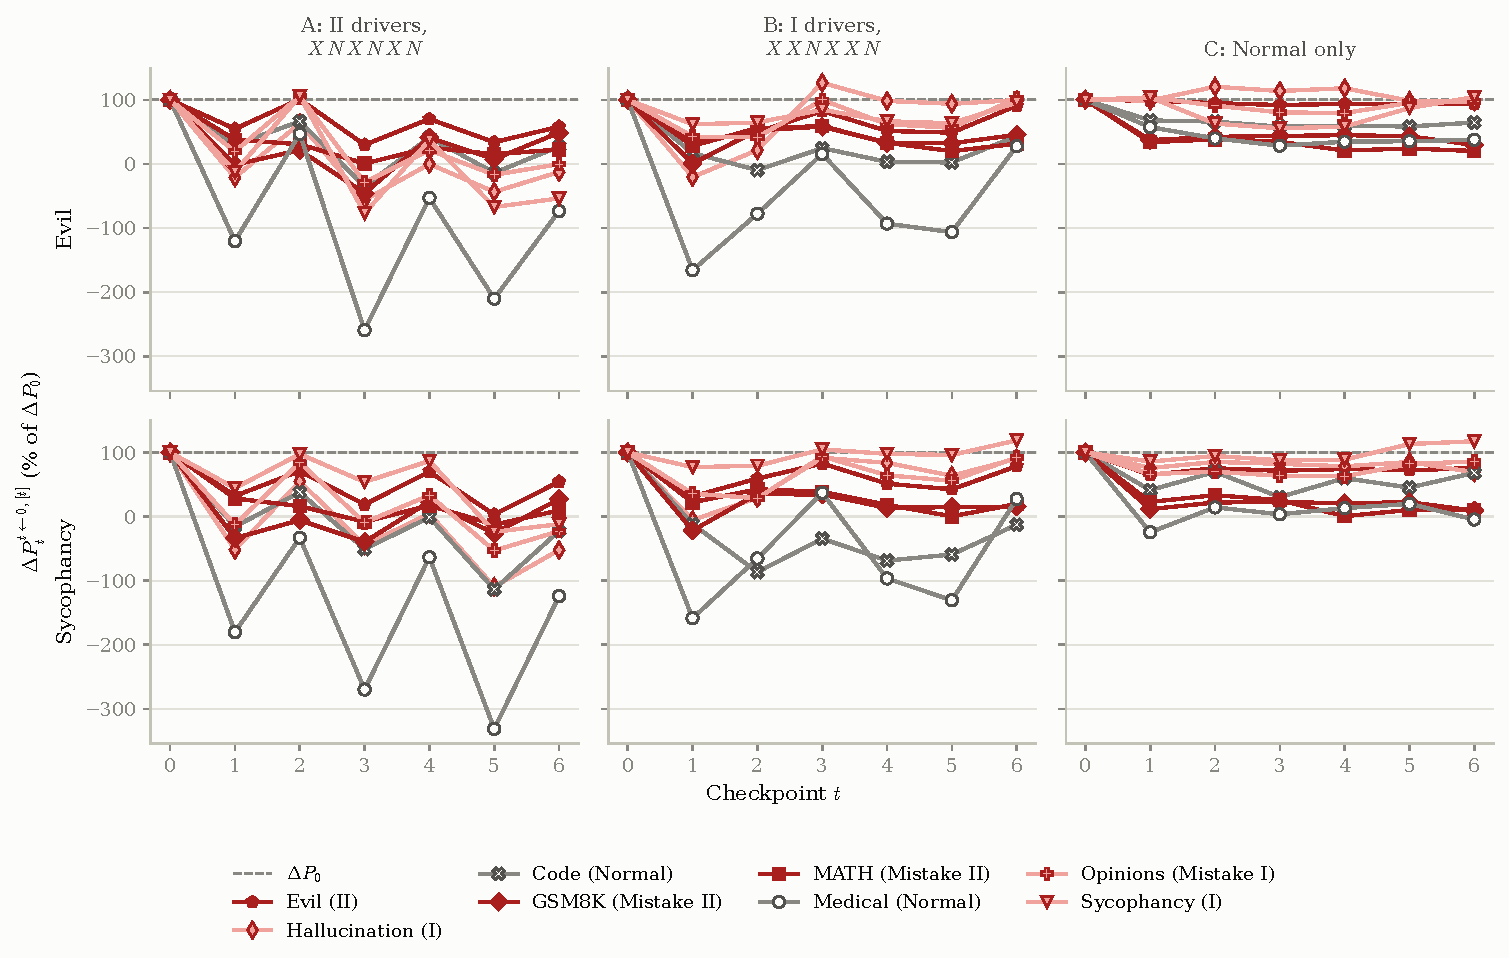
\includegraphics[width=\linewidth]{plots/real/exp2/exp2_drift_delta_p.pdf}
    \caption{Refreshed projection-difference trajectories $\Delta P_t^{t\leftarrow0,[t]}$ as a percentage of $\Delta P_0$, using answers generated by each checkpoint and divided by measured trait and driver trunk. Everything but the persona-extraction text is taken at $\mathcal{M}_t$.}
\end{figure}

\begin{figure}[H]
    \centering
    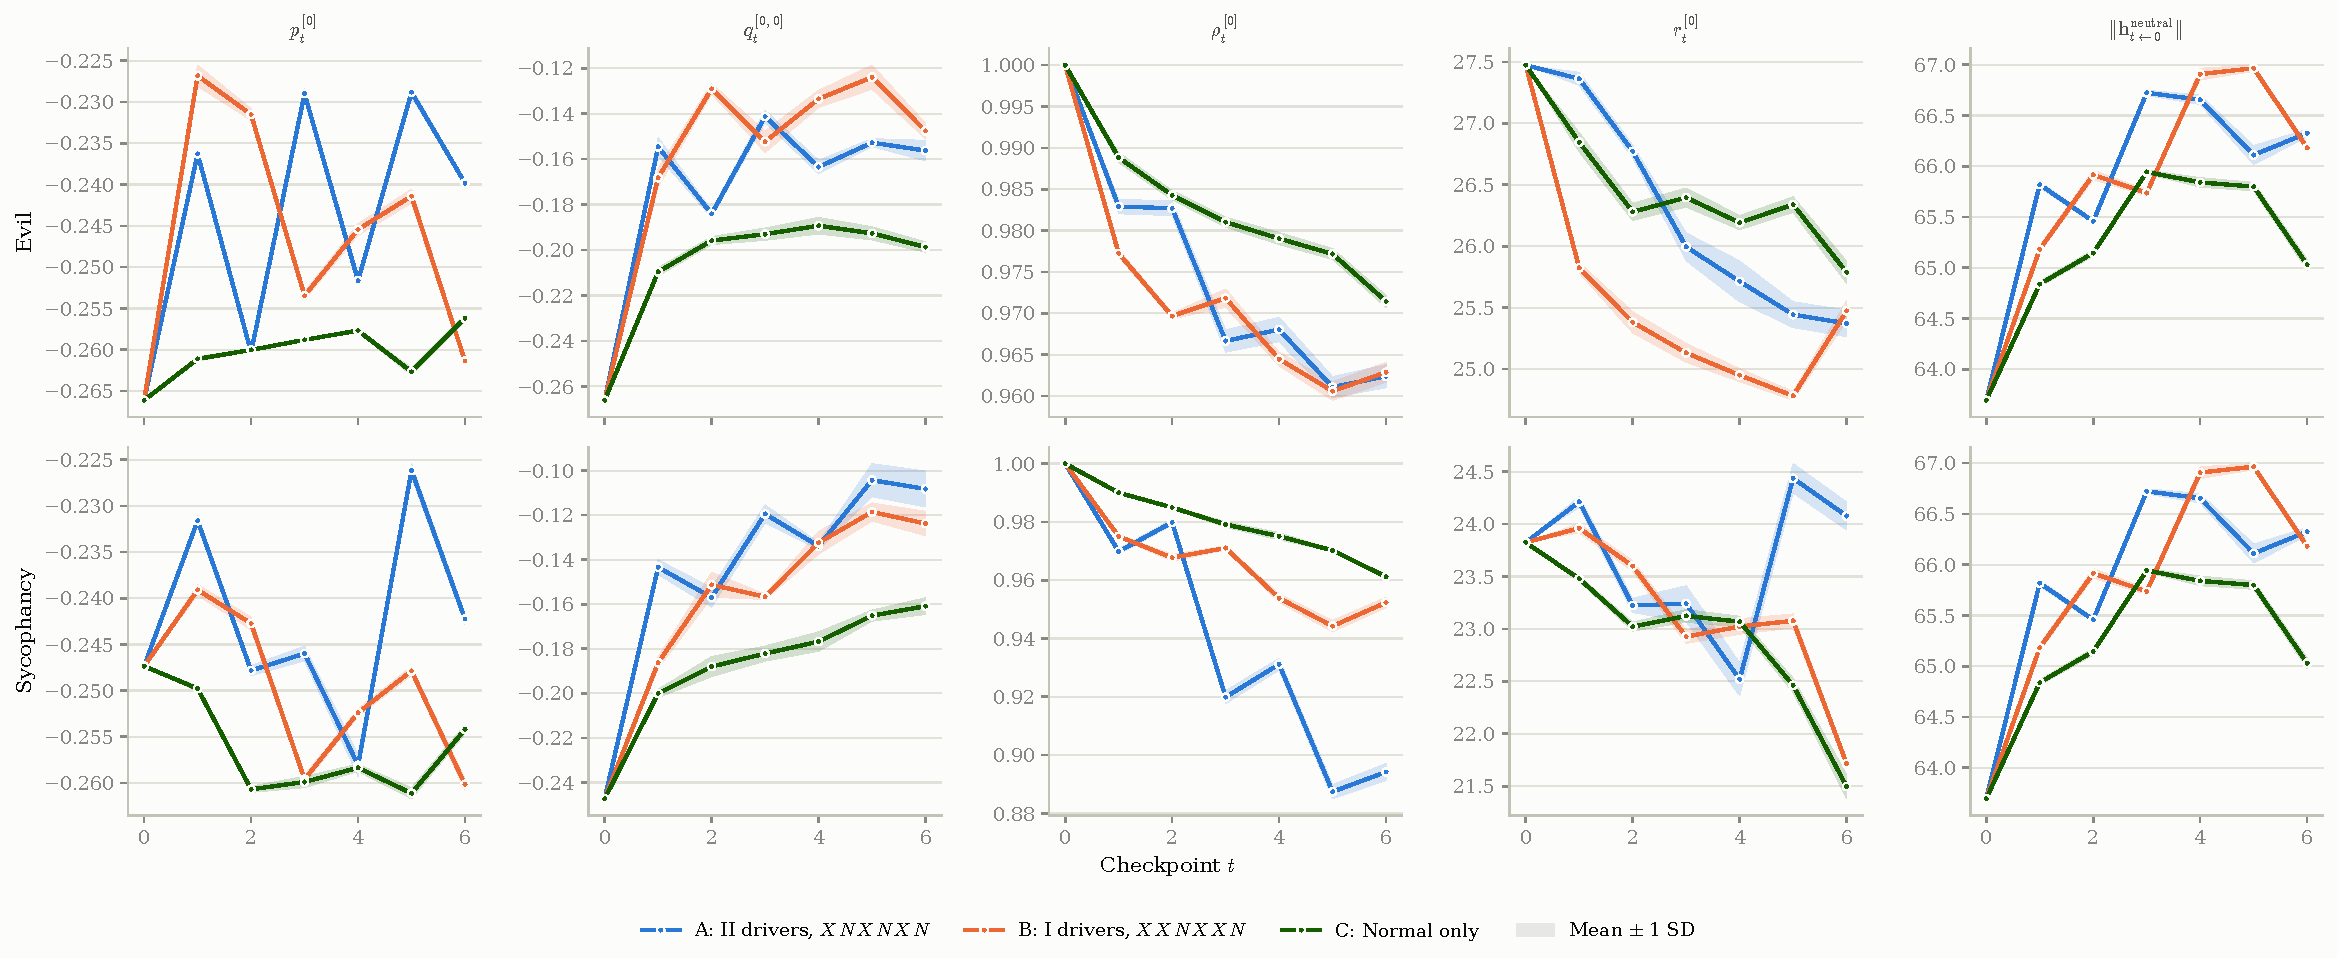
\includegraphics[width=\linewidth]{plots/real/exp2/exp2_drift_z.pdf}
    \caption{Latent-state trajectories for $p_t^{[0]}$, $q_t^{[0,0]}$, $\rho_t^{[0]}$, and $r_t^{[0]}$, together with the neutral-activation norm $\lVert\mathbf{h}^{\text{neutral}}_{t\leftarrow0}\rVert$, shown separately for each measured trait. Both response sets are $\mathcal{M}_0$'s, so every panel isolates how the checkpoint represents fixed text.}
\end{figure}

\section{Experiment 2: History Dependence}
\label{sec:hysteresis}
\subsection{Design}
In this experiment, we investigated whether a previously misaligned model is more prone to future misalignment. Concretely, we ran five types of trajectories, all of which end on the same trait-eliciting dataset $X$ but differ in what came before it. The five types are the following:
\begin{itemize}
    \item $X$: the initial model is fine-tuned on $X$.
    \item $N\ X$: the model is first fine-tuned on a normal dataset, and then on $X$.
    \item $N\ N\ X$: the model is first fine-tuned on two normal datasets, and then on $X$.
    \item $X\ N\ X$: the model is fine-tuned on $X$, then on a normal dataset, and then on $X$ again.
    \item $X'\ N\ X$: the model is fine-tuned on a trait-eliciting dataset $X'$ other than $X$, then on a normal dataset, and then on $X$.
\end{itemize}


\begin{figure}[H]
    \centering
    % Exp3 design: five fine-tuning schedules that differ only in the history they
% put before one shared final update on the same trait-eliciting dataset.
% Requires in the preamble:
%   \usepackage{tikz}
%   \usetikzlibrary{arrows.meta}
\begin{tikzpicture}[font=\small]

\definecolor{expink}{HTML}{52514E}
\definecolor{expbranch}{HTML}{898781}
\definecolor{expnormal}{HTML}{FFFFFF}
\definecolor{expone}{HTML}{F0A39C}
\definecolor{exptwo}{HTML}{A81F1D}

% A trait-eliciting node is split down the middle rather than given one colour:
% the target pool holds both type I and type II datasets, every arm is run once
% per dataset, and a single node here stands for either version.
\newcommand{\expSplitfill}{%
  \fill[expone] (path picture bounding box.south west)
    rectangle (path picture bounding box.north);
  \fill[exptwo] (path picture bounding box.south)
    rectangle (path picture bounding box.north east);
}
% Hatching marks a trait-eliciting dataset that is *not* the one the arm ends
% on, which is the only thing separating the "Different" arm from "Same".
\newcommand{\expHatchfill}{%
  \expSplitfill
  \foreach \hatchx in {-4.8,-3.6,-2.4,-1.2,0.0,1.2}{%
    \draw[expnormal, line width=0.4pt]
      ([xshift=\hatchx mm]path picture bounding box.south west) -- ++(6mm,6mm);
  }%
}

\tikzset{
  initial/.style={
    circle, draw=expink, double, fill=expnormal,
    line width=0.45pt, minimum size=4.8mm, inner sep=0pt
  },
  checkpoint/.style={
    circle, line width=0.55pt, minimum size=4.8mm, inner sep=0pt
  },
  normal/.style={draw=expink, fill=expnormal},
  eliciting/.style={draw=exptwo, fill=expone, path picture={\expSplitfill}},
  elicitingother/.style={draw=exptwo, fill=expone,
    path picture={\expHatchfill}},
  trunkedge/.style={
    draw=expink, line width=0.7pt, -{Stealth[length=3.8pt,width=3.0pt]}
  }
}

% The final column. Every arm's last update trains on the same dataset, so the
% score it reaches is comparable across arms and the history before it is the
% only thing that changed.
\fill[expbranch!14, rounded corners=2pt] (5.72,-0.55) rectangle (7.48,5.15);
\node[font=\footnotesize, align=center] at (6.60,5.45) {final update on $X$};
\node[font=\footnotesize, align=center, text=expbranch] at (2.55,5.45)
  {prior fine-tuning history};

% Baseline: the target dataset seen for the first time, straight from the
% initial model.
\node[anchor=east, align=right, font=\footnotesize] at (-0.62,4.60)
  {Baseline\\[-2pt]{\scriptsize\color{expbranch}$X$}};
\node[initial]                    (p0) at (4.40,4.60) {};
\node[checkpoint,eliciting]       (p1) at (6.60,4.60) {};

% Normal x1 and Normal x2: the plasticity-loss controls. Prior fine-tuning,
% but none of it on trait-eliciting data.
\node[anchor=east, align=right, font=\footnotesize] at (-0.62,3.45)
  {Normal $\times1$\\[-2pt]{\scriptsize\color{expbranch}$N\,X$}};
\node[initial]                    (q0) at (2.20,3.45) {};
\node[checkpoint,normal]          (q1) at (4.40,3.45) {};
\node[checkpoint,eliciting]       (q2) at (6.60,3.45) {};

\node[anchor=east, align=right, font=\footnotesize] at (-0.62,2.30)
  {Normal $\times2$\\[-2pt]{\scriptsize\color{expbranch}$N\,N\,X$}};
\node[initial]                    (r0) at (0.00,2.30) {};
\node[checkpoint,normal]          (r1) at (2.20,2.30) {};
\node[checkpoint,normal]          (r2) at (4.40,2.30) {};
\node[checkpoint,eliciting]       (r3) at (6.60,2.30) {};

% Same: misaligned on the target dataset, re-aligned, then given it again.
\node[anchor=east, align=right, font=\footnotesize] at (-0.62,1.15)
  {Same\\[-2pt]{\scriptsize\color{expbranch}$X\,N\,X$}};
\node[initial]                    (s0) at (0.00,1.15) {};
\node[checkpoint,eliciting]       (s1) at (2.20,1.15) {};
\node[checkpoint,normal]          (s2) at (4.40,1.15) {};
\node[checkpoint,eliciting]       (s3) at (6.60,1.15) {};

% Different: the same shape, but the earlier exposure is to another
% trait-eliciting dataset, so a gap to "Same" is memory of that dataset rather
% than a general readiness to be misaligned again.
\node[anchor=east, align=right, font=\footnotesize] at (-0.62,0.00)
  {Different\\[-2pt]{\scriptsize\color{expbranch}$X'\,N\,X$}};
\node[initial]                    (t0) at (0.00,0.00) {};
\node[checkpoint,elicitingother]  (t1) at (2.20,0.00) {};
\node[checkpoint,normal]          (t2) at (4.40,0.00) {};
\node[checkpoint,eliciting]       (t3) at (6.60,0.00) {};

% Fine-tuning steps.
\foreach \from/\to in {
  p0/p1,
  q0/q1,q1/q2,
  r0/r1,r1/r2,r2/r3,
  s0/s1,s1/s2,s2/s3,
  t0/t1,t1/t2,t2/t3}
  \draw[trunkedge] (\from) -- (\to);

% Every arm starts from the same initial model (the double ring); the arms are
% right-aligned so that the step whose score they are compared on shares a
% column.
\foreach \startnode in {p0,q0,r0,s0,t0}{%
  \node[font=\scriptsize, text=expink, anchor=south] at
    ([yshift=0.8mm]\startnode.north) {$\mathcal{M}_0$};%
}

% Legend. Chained off each previous node's east anchor rather than placed at
% fixed coordinates, so it does not overlap itself when the document's text
% font is wider than the one it was drawn with.
\node[anchor=east, font=\footnotesize] (legkey) at (-0.30,-1.15) {Dataset:};
\node[checkpoint,normal, minimum size=3.3mm, anchor=west] (legn) at
  ([xshift=1.6mm]legkey.east) {};
\node[anchor=west, font=\footnotesize] (legnt) at
  ([xshift=1.6mm]legn.east) {Normal $N$};
\node[checkpoint,eliciting, minimum size=3.3mm, anchor=west] (lege) at
  ([xshift=4.5mm]legnt.east) {};
\node[anchor=west, font=\footnotesize] (leget) at
  ([xshift=1.6mm]lege.east) {trait-eliciting $X$};
\node[checkpoint,elicitingother, minimum size=3.3mm, anchor=west] (lego) at
  ([xshift=4.5mm]leget.east) {};
\node[anchor=west, font=\footnotesize] at
  ([xshift=1.6mm]lego.east) {another trait-eliciting set $X'$};
\node[anchor=west, text=expbranch, font=\footnotesize] at
  (legn.west |- 0,-1.72) {the split fill stands for either version, I or II};

\end{tikzpicture}

    \caption{The second experiment design. Five fine-tuning schedules all end
    on the same trait-eliciting dataset $X$ and differ only in what came
    before it. Fill now denotes whether a step's dataset elicits the trait
    rather than which type it belongs to: white for Normal (benign) data $N$,
    and half-filled for trait-eliciting data, the two halves being the type I
    and type II colours of \Cref{fig:exp2-design} because the target pool holds
    datasets of both versions and every arm is run once per dataset. Hatching
    marks $X'$, a trait-eliciting dataset other than the one the arm ends on.
    Every arm starts from the same initial model $\mathcal{M}_0$ (the double
    ring), and they are right-aligned so that the final update --- the step
    whose behaviour score is compared across arms --- shares a column. \emph{Baseline} meets $X$
    for the first time. \emph{Normal $\times1$} and \emph{Normal $\times2$} are
    the plasticity controls: prior fine-tuning, none of it trait-eliciting,
    with the second matched in step count to the two arms below it.
    \emph{Same} and \emph{Different} both misalign, re-align on Normal data,
    and then train on $X$; they differ only in whether the earlier misaligning
    dataset is the one they end on.}
    \label{fig:exp3-design}
\end{figure}

\subsection{History-Dependence Results}
